\documentclass{beamer}
\usepackage[english]{babel}
\usepackage{geometry}
\usepackage{amsmath}
\usepackage{amsthm}
\usepackage{graphicx}
\usepackage{caption}
\usepackage[utf8]{inputenc}

%%%%%%%% HYPERREF PACKAGE
\hypersetup{colorlinks=true}
\hypersetup{citecolor=orange}
\hypersetup{urlcolor=orange}

%%%%%%%% DEFINITION AND THEOREM DEFINITIONS
\let\definition\relax
\theoremstyle{definition}
\newtheorem{definition}{Definition}[section]

\let\remark\relax
\theoremstyle{remark}
\newtheorem{remark}{Remark}

\theoremstyle{example}
\newtheorem{question}{Question}

%%%%%%%% MULTI-COLUMNS PACKAGE
\usepackage{multicol}

%%%%%%%% BIB-LATEX STUFF
\usepackage[style=authoryear,
            bibstyle=authoryear,
            citestyle=authoryear,
            hyperref=true,
            backend=biber]{biblatex}
\addbibresource{../latex/bib.bib} %Put relative path to ref

%%%%%%%% ICONS FOR CITES
% https://tex.stackexchange.com/questions/68080/beamer-bibliography-icon
\setbeamertemplate{bibliography item}{%
  \ifboolexpr{ test {\ifentrytype{book}} or test {\ifentrytype{mvbook}}
    or test {\ifentrytype{collection}} or test {\ifentrytype{mvcollection}}
    or test {\ifentrytype{reference}} or test {\ifentrytype{mvreference}} }
    {\setbeamertemplate{bibliography item}[book]}
    {\ifentrytype{online}
       {\setbeamertemplate{bibliography item}[online]}
       {\setbeamertemplate{bibliography item}[article]}}%
  \usebeamertemplate{bibliography item}}

\defbibenvironment{bibliography}
  {\list{}
     {\settowidth{\labelwidth}{\usebeamertemplate{bibliography item}}%
      \setlength{\leftmargin}{\labelwidth}%
      \setlength{\labelsep}{\biblabelsep}%
      \addtolength{\leftmargin}{\labelsep}%
      \setlength{\itemsep}{\bibitemsep}%
      \setlength{\parsep}{\bibparsep}}}
  {\endlist}
  {\item}

%%%%%%%% BRACKETS AROUND CITE
% https://tex.stackexchange.com/questions/16765/biblatex-author-year-square-brackets
\makeatletter

\newrobustcmd*{\parentexttrack}[1]{%
  \begingroup
  \blx@blxinit
  \blx@setsfcodes
  \blx@bibopenparen#1\blx@bibcloseparen
  \endgroup}

\AtEveryCite{%
  \let\parentext=\parentexttrack%
  \let\bibopenparen=\bibopenbracket%
  \let\bibcloseparen=\bibclosebracket}

\makeatother

%%%%%%%% THEME SLIDES
\usetheme{default}


%%%%%%%% FRAME TITLES AND SUBTITLES
% https://stackoverflow.com/questions/35810906/vim-beamer-dynamic-frame-title1
\newif\ifinsection
\newif\ifinsubsection

\let\oldsection\section
\renewcommand{\section}{%
  \global\insectiontrue% In section
  \global\insubsectionfalse% Not in subsection
  \oldsection}
\let\oldsubsection\subsection
\renewcommand{\subsection}{%
  %\global\insectionfalse% No in section
  \global\insubsectiontrue% In subsection
  \oldsubsection}

\newcommand {\aframe}[1] {%
  \begin{frame}
    \ifinsection\frametitle{\secname}\fi
    \ifinsubsection\framesubtitle{\subsecname}\fi
  #1
  \end{frame}
}


%%%%%%%% BEAMER STUFF
\setbeamertemplate{footline}[frame number]
\setbeamertemplate{section in toc}[sections numbered]
\setbeamertemplate{subsection in toc}[subsections numbered]
\setbeamertemplate{navigation symbols}{}

%%%%%%%% FOOTNOTE STUFF
\renewcommand{\thefootnote}{\fnsymbol{footnote}}

%%%%%%%% CENTER OF SLIDE THANK YOU
\usepackage{tikz}

\setbeamertemplate{itemize items}[circle]

%%%%%%%% START DOCUMENT
\title{Kalman Filter for Observer-ARMA Model with Parameter Estimation}

\author{Juan Sebasti\'an C\'ardenas-Rodríguez \\ David Plazas Escudero  \\ \vspace{0.5cm} \scalebox{0.7}{Mathematical Engineering, Universidad EAFIT}}

\begin{document}

% Plain so is not numbered
\begin{frame}[plain]
  \titlepage
\end{frame}

%%%%%%%%%% SLIDES %%%%%%%%%%%%%%%
\section{Preliminaries}
\subsection{Notation}
\aframe{
\begin{itemize}
  \item Observed data vector: $y^*_t:=(y_0^T,\,y_1^T,\dots,y_t^T)^T$.
  \item $z_{t|t-1}:=E(z_t|y^*_{t-1})$ and $y_{t|t-1}:=E(y_t|y^*_{t-1})$.
  \item $\Delta y_t:=y_t-y_{t|t-1}$ and $\Delta z_t:=z_t-z_{t|t-1}$.
  \item $\Sigma_{t|t}:=\text{Cov}(\Delta z_t|y_t^*$).
\end{itemize}
}

\subsection{Observer-ARMA Model}
\aframe{
The general scheme for the observer-ARMA model is given by
\begin{equation}
  \begin{split}
    &z_{t+1}=\sum_{s=0}^{l_1}a_sz_{t-s}+\sum_{s=0}^{l_2}b_s\xi_{t-s}\\
    &y_t=h_tz_t+\zeta_t\\
    &z_0,z_{-1},\ldots,z_{-l_1}\in \mathbb{R}, \ t=0,1,\ldots
  \end{split}
\end{equation}
}

\subsection{Kalman Filter}
\aframe{
  The standard KF Procedure \parencite{kalman1960new} has two main hypothesis:\\
  \textbf{H1}
  \[
  \begin{split}
  &E(\xi_t)=E(\zeta_t)=0, \quad t=0,1,\ldots\\
  &E(\xi_t\xi_t^T)=Q_t, \quad E(\zeta_t\zeta_t^T)=R_t\\
  &E(\xi_t\xi_s^T)=E(\zeta_t\zeta_s^T)=0,\quad\forall s\neq t\\
  &E(\xi_t\zeta_s^T)=0, \quad \forall t,s=0,1,\ldots\\
  &E(z_tz_s^T)=0,\quad\forall t\neq s
  \end{split}
  \] \pause

  \textbf{H2}
  \[\xi_t\sim\mathcal{N}(0,Q_t),\quad\zeta_t\sim\mathcal{N}(0,R_t),\quad\forall t=0,1,\ldots\]
}

\aframe{
The KF procedure is now presented:
\begin{enumerate}
  \item \textbf{Initialization: }
  \[
  z_{0|0}=z_0\in \mathbb{R}^n, \ \Sigma_{0|0}=0
  \]
  \item \textbf{Prediction: }
  \[
  \begin{split}
    &z_{t|t-1}=F_tz_{t-1|t-1}\\
    &\Sigma_{t|t-1}=F_{t-1}\Sigma_{t-1|t-1}F_{t-1}^T+Q_{t-1}
  \end{split}
  \]
  \item \textbf{Correction: }
  \[
  \begin{split}
    &z_{t | t}=z_{t | t-1}+M_{t}^{\text{opt}} \Delta y_{t} \\
    &\Sigma_{t | t}=\Sigma_{t | t-1}-M_{t}^{\text{opt}} H_{t} \Sigma_{t | t-1}
  \end{split}
  \]
  where ${M_{t}^{\text {opt}}=\Sigma_{t | t-1} H_{t}^{T}\left(H_{t} \Sigma_{t | t-1} H_{t}^{T}+R_{t}\right)^{-1}}$.
\end{enumerate}
}

\subsection{Extended Kalman Filter}
\aframe{
  Let $f:\mathbb{R}^n \rightarrow \mathbb{R}^n$ be a given vector function.
\begin{equation}
  \begin{cases}
    x_{t+1}=f(x_t) + \xi_t&\\
    y_t=H_tx_t+\zeta_t&\\
    x_0\in \mathbb{R}^n, \ t=0,1,\ldots &
  \end{cases}
  \pause \implies
  \begin{cases}
    x_{t+1}=\tilde{F}x_t + \xi_t&\\
    y_t=H_tx_t+\zeta_t &\\
    x_0\in \mathbb{R}^n, \ t=0,1,\ldots &
  \end{cases}
\end{equation}
Where $\tilde{F}$ is:
\[
\tilde{F}:=\dfrac{\partial f(t,x)}{\partial x}\bigg|_{x=x^{{\rm ref}}_t}
\]
}

\section{Instrumental Extended Kalman Filter}
\subsection{Problem Definition}
\aframe{
In this work we will use a simple ARMA model, with correlated state and one unknown stationary parameter $a$. The model in consideration is
\begin{equation}
  \begin{split}
    &z_{t+1}=az_t+\xi_t+d\xi_{t-1}\\
    &y_{t}=hz_t+\gamma_{t}\\
    &z_0\in\mathbb{R}, \ t=0,1,\dots
  \end{split}
\end{equation}
\pause
\begin{remark}
  The objective is find an estimator $\tilde{a}$ for the unknown parameter $a$ using the data vector $y^*_t$.
\end{remark}
}

\subsection{Assumptions}
\aframe{
  It is assumed that the parameter $\tilde{a}$ is not constant, even if the original parameter is. \\ \vspace{0.5cm} \pause

  It is supposed that $\tilde{a}$ behaves as:
\begin{equation}
  \tilde{a}_t=b\tilde{a}_{t-1}+\chi_{t-1}
\end{equation}
with $0<b<1$ and $\chi_t \sim N(0,\,\sigma)$.
}

\subsection{Final Model}
\aframe{
Given the dynamics for $\tilde{a}_t$, we propose the complete dynamics for the ARMA model as
\begin{equation}\label{eq:mainARMA}
  \begin{split}
    &z_{t+1}=\tilde{a}_tz_t+\xi_t+d\xi_{t-1}\\
    &\tilde{a}_{t+1}=b\tilde{a}_t+\chi_t\\
    &z_0, \, \tilde{a}_0\in\mathbb{R},\,t=0,1,\dots
  \end{split}
\end{equation} \pause

Let $x_t:=(z_t,\,\tilde{a}_t)^T$ and $x^{{\rm ref}}_t:=(z_t^{{\rm ref}},\,\tilde{a}_t^{{\rm ref}})^T$. Extended Kalman Filter is applied.
\[
\tilde{F}_t = \begin{bmatrix}
\tilde{a} & z\\
0 & b
\end{bmatrix}_{x=x_t^{{\rm ref}}}
\]
}

\aframe{
  Let $\tilde{x}_t:=x_{2t}$, these transformation assures that the new state $\tilde{x}_t$ is not correlated with $\tilde{x}_{t-1}$.
  \[\tilde{y}_t^*:=\begin{cases}
   (y_0^T, y_2^T,\ldots,y_t^T)^T,&t\text{ even}\\
   (y_0^T, y_2^T,\ldots,y_{t-1}^T)^T,&t\text{ odd}
 \end{cases}\]
Now, given the instrumental variables transformation and the linearization procedure for model, the standard KF procedure can be applied.
}

\section{Discussion \& Future Work}

\aframe{
  \begin{figure}[H]
    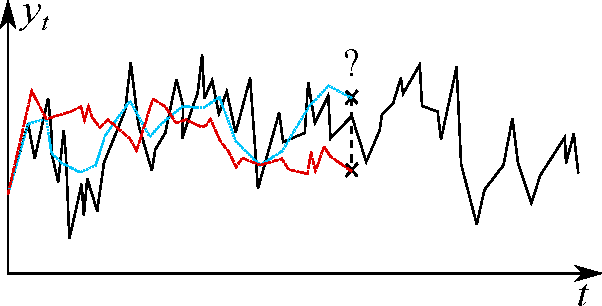
\includegraphics[scale=1]{drawing.pdf}
  \end{figure}
}

%%%%%%%%%%%%%%%%%%%%%%%%%%%%%%%%%
\begin{frame}[allowframebreaks]{References}
  \printbibliography
\end{frame}

\begin{frame}
  \begin{tikzpicture}[overlay, remember picture]
     \node[anchor=center] at (current page.center) {
     \Huge{\emph{Thank you}}};
\end{tikzpicture}
  \begin{minipage}[t][.8\textheight]{\textwidth}
    \vfill
    \begin{center}
          \begin{multicols}{2}
            \scalebox{0.7}{\textbf{Student Contact}} \\
            \scalebox{0.7}{Juan Sebasti\'an C\'ardenas-Rodríguez} \\
            \scalebox{0.7}{jscardenar@eafit.edu.co} \\

            \columnbreak
            \scalebox{0.7}{\textbf{Student Contact}} \\
            \scalebox{0.7}{David Plazas Escudero} \\
            \scalebox{0.7}{dplazas@eafit.edu.co}
    \end{multicols}
    \end{center}
  \end{minipage}
\end{frame}

\end{document}
